\documentclass[kulak]{kulakarticle}

\usepackage{amsmath}
\usepackage{amssymb}
%\usepackage{amsfonts}
%\usepackage{amsthm}
%\usepackage{tcolorbox}
\usepackage{mathtools}
\usepackage{siunitx}
\usepackage{cancel}
%\usepackage{mathtools}
\usepackage[american, straightlabels, cuteinductors]{circuitikz}
\usepackage{subcaption}

%\DeclareUnicodeCharacter{}{I~AM~HERE!!!!}

\let\epsilon\varepsilon

\newcommand{\R}{\mathbb{R}} % Real numbers
\newcommand{\C}{\mathbb{C}} % Complex numbers
\newcommand{\Q}{\mathbb{Q}}
\newcommand{\N}{\mathbb{N}}

\DeclarePairedDelimiter\abs{\lvert}{\rvert}
\usepackage{array}
\usepackage{multirow}

\sisetup{output-decimal-marker={.}}
\sisetup{per-mode=symbol}
\sisetup{per-symbol=/}
\sisetup{group-digits=integer}

\newcommand{\rood[1]}{\color{red}#1\color{black}}

\usepackage[dutch]{babel}
\usepackage{hyperref}

%\setlength{\parindent}{0pt}
% d voor dx
\newcommand*\diff{\mathop{}\!\mathrm{d}}

\usepackage{parskip}

\title{Examen Elektrische Netwerken}
\author{Vincent Van Schependom}
\date{20 januari 2025}
\address{
	\textbf{Elektrische Netwerken}\\
	Ben Hermans}

\begin{document}

	\maketitle

	\section*{Vraag 2}

	\vspace{-0.5cm}
	\begin{figure}[h!]
		\centering
		\begin{subfigure}{.49\textwidth}
			\centering
				\begin{tikzpicture}
				\draw (0,0) to[short, *-, R, l=$R_1$] (0,2.5) node[](links){}
				to[short, *-] (0,3) node[](linksonder){}
				to[short, *-, I, l=$I_S$] ++ (3,0) node[](is){}
				to[short, *-] ++ (3,0);
				\draw (linksonder.center) 	to [*-, R, l=$R_2$] ++ (0,3) node[](linksboven){}
				to [*-, C, l=$C$] (is.center)
				to [*-, R, l=$R$] ++ (0,3);
				\draw (linksboven.center) to [short, *-, L, l=$L$] ++ (3,0)
				to [short, *-] ++ (3,0) node[](rechtsboven){}
				to [short, *-*, controlled current source, invert, l=$\alpha i_{R_1}$] ++ (0, -3) node[](rechtsonder){} to[short, -*] ++ (0,-0.5) node[](rechts){};
				\draw (3,6) to [short, *-, controlled isource, invert, l=$\beta v_{R_2}$, label position=above] ++ (3,-3);

				\node[draw, circle, minimum size=1cm] (raarelement) at (3,1) {};
				\draw (links.center) to[short] (raarelement.145) to[short] (raarelement.center);
				\draw (rechts.center) to[short] (raarelement.35) to[short] (raarelement.center);
				\draw (raarelement.center) to[short, -*] ++(0,-1) node[](middenonder){};

				\draw (0,0) to[short] (middenonder.center)
								to[short, *-*] ++ (3,0)
								to[short, -] ++ (0,0.25)
								to[short, -, vsource, invert, v_=$v_4$] ++ (0,1)
								to[short, -, vsource, invert, v_=$v_3$] ++ (0,1)
								to[short, -*] ++ (0,0.25);

			\end{tikzpicture}
			\caption{}
			\label{fig:a}
		\end{subfigure}
		\hfill
		\begin{subfigure}{.49\textwidth}
			\centering
			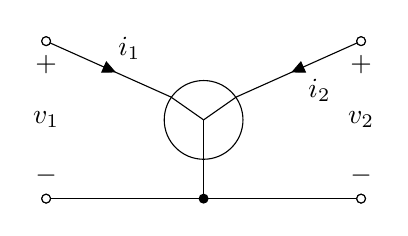
\begin{tikzpicture}

				\node[draw, circle, minimum size=1cm] (raarelement) at (2,1) {};

				\draw (0,2) node[](linksboven){} to[short, o-, i=$i_1$] (raarelement.145) to[short] (raarelement.center);
				\draw (4,2) node[](rechtsboven){} to[short, o-, i=$i_2$] (raarelement.35) to[short] (raarelement.center);
				\draw (raarelement.center) to[short, -*] ++(0,-1) node[](middenonder){};

				\draw (0,0) node[](linksonder){} to[short, o-] (middenonder.center)
				to[short, -o] ++ (2,0) node[](rechtsonder){};

				\draw (linksboven) to[open, o-o, v=$v_1$] (linksonder);
				\draw (rechtsboven) to[open, o-o, v=$v_2$] (rechtsonder);

			\end{tikzpicture}
			\caption{}
			\label{fig:b}
		\end{subfigure}
	\end{figure}

	Voer Modified Node Analysis uit op het circuit in (a), waarbij de karakteristiek van de tweepoort in (b) gegeven wordt door: \begin{align*}
		\begin{cases}
			v_1 = 6i_1 + 2i_2\\
			v_2 = 4i_1 + 3i_2
		\end{cases}
	\end{align*}
	Geef duidelijk aan wat je (niet) met gewone knooppuntanalyse kan bepalen.

	\newpage

	\newpage

	\section*{Vraag 3}

	\begin{figure}[h!]
		\centering
		\begin{circuitikz}
	\draw   (0,0) node[transformer] (T) {};

	% Input and output nodes
	\draw (T.A1) node[anchor=east, ocirc] (i) {}
	(T.A2) node[anchor=east, ocirc] (j) {}
	(T.B1) node[anchor=west, ocirc] (m) {}
	(T.B2) node[anchor=west, ocirc] (k) {};

	% Labels near terminals
	\draw (i) ++ (-0.15,0) node[anchor=east, circle, draw] {$i$}
	(j) ++ (-0.15,0) node[anchor=east, circle, draw] {$j$}
	(m) ++ (0.15,0) node[anchor=west, circle, draw] {$m$}
	(k) ++ (0.15,0) node[anchor=west, circle, draw] {$k$}

	% Transformer ratio label
	(T.base) node[above] {$n:1$};
\end{circuitikz}
	\end{figure}

	Beschouw de ideale transformator hierboven.

	\begin{enumerate}
		\item[a)] Welke beschrijvingen bestaan?
		\item[b)] Kunnen we deze component beschrijven met behulp van gewone knooppuntanalyse?
		\item[c)] Leid de stempel van de ideale transformator af.
	\end{enumerate}

	\newpage

	\section*{Vraag 4}
	\vspace{-0.8cm}
	\begin{figure}[h!]
		\centering
		\begin{circuitikz}
			\draw (0,0) node[] (top) {} to[short, o-*, C, l_=$C$, i>_=$i$] ++ (-1.5,0) node[] (weerstand3) {}
						to[short, -*] ++ (-1,0) node[] (weerstand2) {}
						to[short, -*] ++ (-1.5,0) node[] (source) {}
						to[short, -] ++ (-0.5,0)
						to[short, R, l=$R_1$] ++ (-1.5,0)
						to[short, L, l=$L$] ++ (-1.5,0)
						to[short, -] ++ (-0.5,0)
						to[short, vsource, l=$E_0$] ++ (0,-3)
						to[short, -o] ++ (8,0) node[] (bottom) {};

			\draw (weerstand2.center) to[R,l_=$R_2$] ++ (0,-3);
			\draw (weerstand3.center) to[R,l=$R_3$] ++ (0,-3);
			\draw (source.center) to[controlled isource,l_=$2I$] ++ (0,-3);

			\draw (top) to[open, v=$v$] (bottom);
		\end{circuitikz}
	\end{figure}

	Teken het fasorendiagram van bovenstaand netwerk, ervan uitgaande dat \(I\neq 0\). De complexe amplitudes van \(E_0\) en \(I\) zijn respectievelijk \SI{2}{\volt} en \(\sqrt{2}\,\SI{}{\ampere}\).

	\vspace{1cm}

	\begin{figure}[h!]
		\centering
		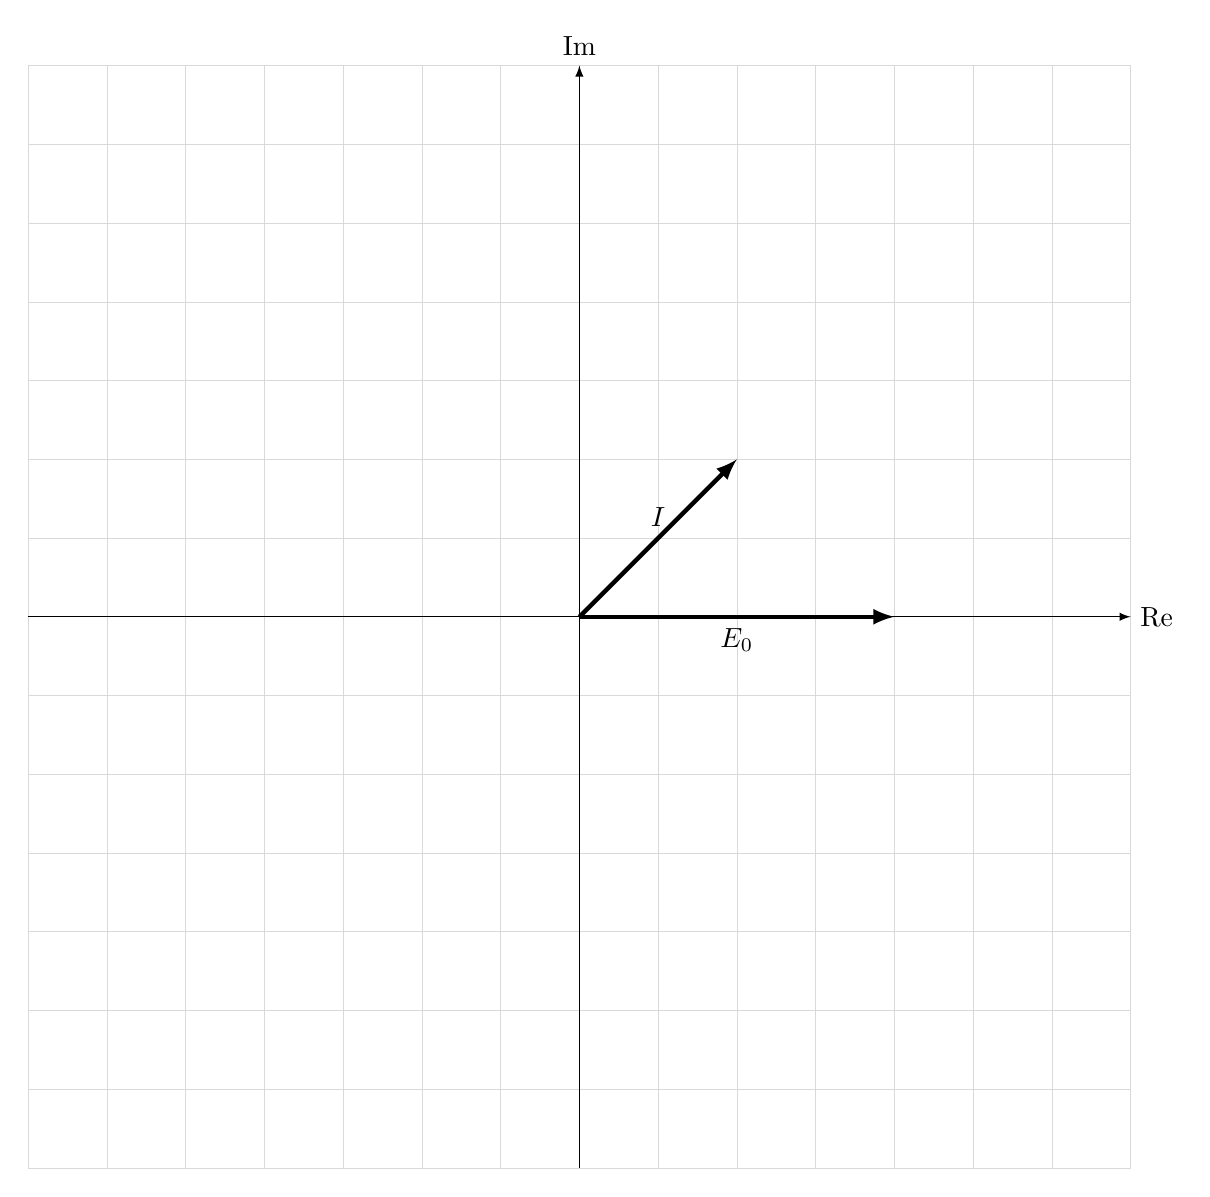
\begin{tikzpicture}
			\draw[help lines, color=gray!30] (-7,-7) grid (7,7);
			\draw[-latex] (-7,0)--(7,0) node[right]{Re};
			\draw[-latex] (0,-7)--(0,7) node[above]{Im};
			\draw[ultra thick, -latex] (0,0)--(2,2) node[midway,above] () {$I$};
			\draw[ultra thick, -latex] (0,0)--(4,0) node[midway,below] () {$E_0$};
		\end{tikzpicture}
	\end{figure}

	\newpage

	\section*{Vraag 5}

	\begin{figure}[h!]
		\centering
		\begin{subfigure}{.4\textwidth}
			\centering
			\begin{circuitikz}
				\draw (0,0) node[] (linksonder) {} to[short, o-] ++ (2,0)
				to[short, -*] ++ (0,1) node[] (onder) {};

				\draw (onder.center) 	to[short] ++ (-1,0)
				to[short] ++ (0,0.5)
				to[R, l=$\SI{1}{\ohm}$] ++ (0,1.5)
				to[diode, invert] ++ (0,1.5)
				to[short] ++ (0,0.5);

				\draw (onder.center) 	to[short] ++ (1,0)
				to[isource, l=$\SI{2}{\ampere}$] ++ (0,4)
				to[short, -*] ++ (-1, 0) node[] (boven) {}
				to[short] ++ (-1,0);

				\draw(boven.center) to[short, i=$i$] ++ (0,1)
				to[short, -o] ++ (-2,0) node[] (linksboven) {};

				\draw(linksboven) to [open, v=$v$] (linksonder);
			\end{circuitikz}
			\subcaption{}
		\end{subfigure}
		\hspace{.2cm}
		\begin{subfigure}{.4\textwidth}
			\centering
			\begin{circuitikz}[ bigR/.style={ageneric, bipoles/length=2cm, v^>={$v=f(i)$}} ]

				\draw (0,0) node[] (linksonder) {} to[short] ++ (5,0)
				to[short, -*] ++ (0,1) node[] (onder) {};

				\draw (onder.center) 	to[short] ++ (-1,0)
				to[short] ++ (0,0.5)
				to[R, l=$\SI{1}{\ohm}$] ++ (0,1.5)
				to[diode, invert] ++ (0,1.5)
				to[short] ++ (0,0.5);

				\draw (onder.center) 	to[short] ++ (1,0)
				to[isource, l=$\SI{2}{\ampere}$] ++ (0,4)
				to[short, -*] ++ (-1, 0) node[] (boven) {}
				to[short] ++ (-1,0);

				\draw(boven.center) to[short] ++ (0,1)
				to[short, -] ++ (-5,0) node[] (linksboven) {}
				to[short,i>_=$i$] ++ (0,-1.5)
				to[bigR] ++ (0, -3)
				to[short] ++ (0,-1.5);
			\end{circuitikz}
			\subcaption{}
		\end{subfigure}
	\end{figure}

		De karakteristiek van het niet-lineair element in het netwerk in (b) is gelijk aan \begin{align*}
		R_g = \{(v,i) \mid e^{-v} - 2v + 2i =0 \}.
	\end{align*}

	\begin{enumerate}
		\item[a)] Bepaal visueel de \((v,i)\)-karakteristiek van de tweeterminal in (a) en teken deze karakteristiek op Figuur \ref{fig:nietlineair}.
		\item[b)] Bepaal ongeveer de oplossing van het netwerk in (b).
		\item[c)] Lineariseer de niet-lineaire component in \(v^{(0)}=\SI{1}{\volt}\).
		\item[d)] Voer één Newton-Raphson iteratie uit.
	\end{enumerate}

	\vspace{1cm}

	\begin{figure}[h!]
		\centering
		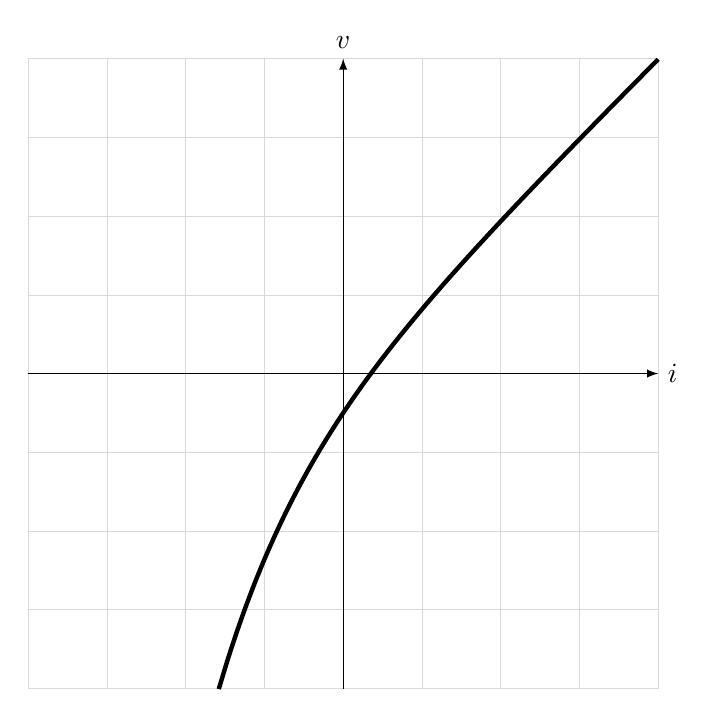
\begin{tikzpicture}
			\draw[help lines, color=gray!30] (-4,-4) grid (4,4);
			\draw[-latex] (-4,0)--(4,0) node[right]{$i$};
			\draw[-latex] (0,-4)--(0,4) node[above]{$v$};
			\draw[ultra thick,black] plot[domain=-1.58:4, samples = 50, smooth]({\x}, {-(1/2)*exp(-\x)+\x});
		\end{tikzpicture}
		\caption{De \((v,i)\)-karakteristiek van de niet-lineaire weerstand.}
		\label{fig:nietlineair}
	\end{figure}

\end{document}


























